\documentclass{iaesarticle}

%%required package. add for your convenient, but do not remove the initial
\setlength{\headsep}{0.15in}
\usepackage{amsmath, amsfonts, amssymb, float, fancyhdr}
\usepackage[figuresright]{rotating}
\usepackage{authblk, graphicx, indentfirst, lastpage, lipsum}
\usepackage{pifont}
\renewcommand{\Authsep}{, }
\renewcommand{\Authand}{, }
\renewcommand{\Authands}{, }
\setlength{\affilsep}{0cm}
\renewcommand\Authfont{\normalsize}
\renewcommand\Affilfont{\fontsize{8}{10}\mdseries}
\makeatletter
\renewcommand{\@biblabel}[1]{[#1]\hfill}
\renewcommand\AB@authnote[1]{\textsuperscript{\normalfont\bfseries#1}}
\makeatother
\usepackage[font=normalsize=]{subfig, caption}
\usepackage{epstopdf}
\usepackage[left=3cm, right=2.5cm, top=2.5cm, bottom=2.5cm, includehead, includefoot]{geometry}
\usepackage[justification=centering]{caption}
\captionsetup{labelsep=period}
\usepackage{titlesec}
\usepackage[table]{xcolor}
\titleformat{\section}
{\normalfont\normalsize\bfseries\uppercase}{\thesection}{1.7em}{} 
\titleformat{\subsection}
{\normalfont\normalsize\bfseries}{\thesubsection}{.95em}{}
\titleformat{\subsubsection}
{\bfseries}{\thesubsubsection}{.2em}{}
\titlespacing*{\section}{0cm}{0.7cm}{0cm}
\usepackage{enumitem}
\usepackage[numbers,sort&compress]{natbib}
\usepackage{ragged2e}
\usepackage{hyperref,graphicx}
\usepackage{multirow}
\usepackage{fleqn}


%%leave copyright info to the editor
\CopyrightLine[]{}{\textit{This is an open access article under the \textcolor{blue}{\underline{CC BY-SA}} license.}
\vspace{.5em}}

%%author
\author[1]{\bfseries Zahra Pezeshki}
\author[2]{\bfseries Tanweer Alam}
\author[3,4]{\bfseries Laith Mohammad Abualigah}

%%author's affiliation
\affil[1]{Department Electrical Engineering-Electronics Integrated Circuits, Faculty of Electrical and Robotics Engineering, \linebreak Shahrood University of Technology, Shahrood, Semnan, Iran}
\affil[2]{Department of Computer Science, Faculty of Computer and Information Technology, Islamic University of Madinah, \linebreak Medina, Saudi Arabia }
\affil[3]{Department of Software Engineering, Faculty of Computer Sciences and Informatics, Amman Arab University, Amman, Jordan}
\affil[4]{School of Computer Sciences, Universiti Sains Malaysia (USM), Gelugor, Pulau Pinang, Malaysia}

%%title and shortitle (for footer)
\title{Paper’s title should be the fewest possible words that accurately describe the content of the paper}
\shorttitle{Paper’s should be the fewest possible that accurately describe … (First Author)}

%%starting
\begin{document}
\setcounter{page}{1}

%%indentation. do not change
\setlength{\parindent}{1.27cm}

%%header and footer setting. do not change
\pagestyle{fancy}
\fancyhfoffset{0cm}

%%journal info
\journalname{Computer Science and Information Technologies}
\journalshortname{Comput Sci Inf Technol}
\journalhomepage{http://iaesprime.com/index.php/csit}
\vol{99}
\no{1}
\months{Month}
\years{2099}
\issn{2722-3221}
\DOI{10.11591}
\pagefirst{1}
\pagelast{1x}

%%build title
\maketitle

%%border setting. do not change
\hrule
\vspace{.1em}
\hrule
\vspace{.5em}
\noindent
\parbox[t][][s]{0.315\textwidth}{%
\textbf{Article Info}
\vspace{.5em}
\hrule
\vspace{.5em}
\begin{history}
\vspace{.5em}

%%article info. editor's privilege
Received month dd, yyyy

Revised month dd, yyyy

Accepted month dd, yyyy

\vspace{.7em}
\end{history}
\vspace{.5em}
\hrule
\vspace{.5em}
\begin{keyword} 
\vspace{.5em}
%%write keyword here. separate by \sep
First keyword \sep Second keyword \sep Third keyword \sep Fourth keyword \sep Fifth keyword
\vspace{.5em}
\end{keyword}
\vspace{\fill}
}
\parbox{0.020\textwidth}{\hspace{.5em}}
\parbox[t][][s]{0.65\textwidth}{%
\begin{abstract}
\vspace{.3em}
%% Text of abstract
An abstract is often presented separate from the article, so it must be able to stand alone. A well-prepared abstract enables the reader to identify the basic content of a document quickly and accurately, to determine its relevance to their interests, and thus to decide whether to read the document in its entirety. The abstract should be informative and completely self-explanatory, provide a clear statement of the problem, the proposed approach or solution, and point out major findings and conclusions. \textbf{The Abstract should be 100 to 200 words in length}. References should be avoided, but if essential, then cite the author(s) and year(s). Standard nomenclature should be used, and non-standard or uncommon abbreviations should be avoided, but if essential they must be defined at their first mention in the abstract itself. No literature should be cited. The keyword list provides the opportunity to add 5 to 7 keywords, used by the indexing and abstracting services, in addition to those already present in the title.
\end{abstract}
}
\parbox[l]{\textwidth}{%
\rule{0.275\textwidth}{0.5pt} \hspace{0.5cm} \hrulefill
\\
\emph{\textbf{Corresponding Author:}}
\vspace{.5em}\\
%% correspondence info. separate by \\
Laith Mohammad Abualigah\\
Department of Software Engineering, Faculty of Computer Sciences and Informatics,
Amman Arab University\\
Jordan street, Amman, Jordan\\
Email: ojugo.arnold@fupre.edu.ng
}
\vspace{.5em}
\hrule
\vspace{.1em}
\hrule


%% main text

\section{Introduction}
\label{}
The main text format consists of flat left-right columns on A4 paper (quarto). The margin text from the left and top are 2.5 cm, right and bottom are 2 cm. The manuscript is written in Microsoft Word, single space, Time New Roman 10 pt, and maximum 12 pages for original research article, or maximum 16 pages for review/survey paper, which can be downloaded at the website: http://iaesprime.com/index.php/csit.

The title of an article should consist of the fewest possible words that accurately describe the content of the paper. The title should be succinct and informative and no more than about 12 words in length. Do not use acronyms or abbreviations in your title and do not mention the method you used, unless your paper reports on the development of a new method. Titles are often used in information-retrieval systems. Avoid writing long formulas with  subscripts in the title.. Omit all waste words such as \textit{"A study of ...", "Investigations of ...", "Implementation of ...”, "Observations on ...", "Effect of.....", “Analysis of …”}, “Design of…” etc. 

A concise and factual abstract is required. The abstract should state briefly the purpose of the research, the principal results and major conclusions. An abstract is often presented separately from the article, so it must be able to stand alone. For this reason, References should be avoided, but if essential, then cite the author(s) and year(s). Also, non-standard or uncommon abbreviations should be avoided, but if essential they must be defined at their first mention in the abstract itself. Immediately after the abstract, provide a maximum of 7 keywords, using American spelling and avoiding general and plural terms and multiple concepts (avoid, for example, 'and', 'of'). Be sparing with abbreviations: only abbreviations firmly established in the field may be eligible. These keywords will be used for indexing purposes. Indexing and abstracting services depend on the accuracy of the title, extracting from it keywords useful in cross-referencing and computer searching. An improperly titled paper may never reach the audience for which it was intended, so be specific. 

The Introduction section should provide: i) a clear background, ii) a clear statement of the problem, iii) the relevant literature on the subject, iv) the proposed approach or solution, and v) the new value of research which is innovation (within 3-6 paragraphs). It should be understandable to colleagues from a broad range of scientific disciplines. Organization and citation of the bibliography are made in Institute of Electrical and Electronics Engineers (IEEE) style in sign [1], [2] and so on. The terms in foreign languages are written italic (italic). The text should be divided into sections, each with a separate heading and numbered consecutively [3]. A full article usually follows a standard structure: \textbf{1. INTRODUCTION, 2. THE COMPREHENSIVE THEORETICAL BASIS AND/OR THE PROPOSED METHOD/ALGORITHM} (optional), \textbf{3. METHOD, 4. RESULTS AND DISCUSSION, and 5. CONCLUSION.} The structure is well-known as \textbf{IMRaD} style.

Literature review that has been done author used in the section \textbf{INTRODUCTION} to explain 
the difference of the manuscript with other papers, that it is innovative, it are used in the section \textbf{METHOD} to describe the step of research and used in the section \textbf{RESULTS AND DISCUSSION} to support the analysis of the results [2]. If the manuscript was written really have high originality, which proposed a new method or algorithm, the additional section after the \textbf{INTRODUCTION} section and before the \textbf{METHOD} section can be added to explain briefly the theory and/or the proposed method/algorithm [4].


\section{METHOD}
\label{}
Explaining the research chronologically, including the research design, research procedures (in the form of algorithms, Pseudocode, or other), how to test, and data acquisition [5]–[7]. The description of the course of research should be supported references, so the explanation can be accepted scientifically [2], [4]. Figures 1-2 and Table 1 are presented center, as shown below and cited in the manuscript [5], [8]–[13]. Tenant placement for effectiveness as shows in Figure 2(a) and for scalability as shows in Figure 2(b).

\begin{figure}[H]
\centering
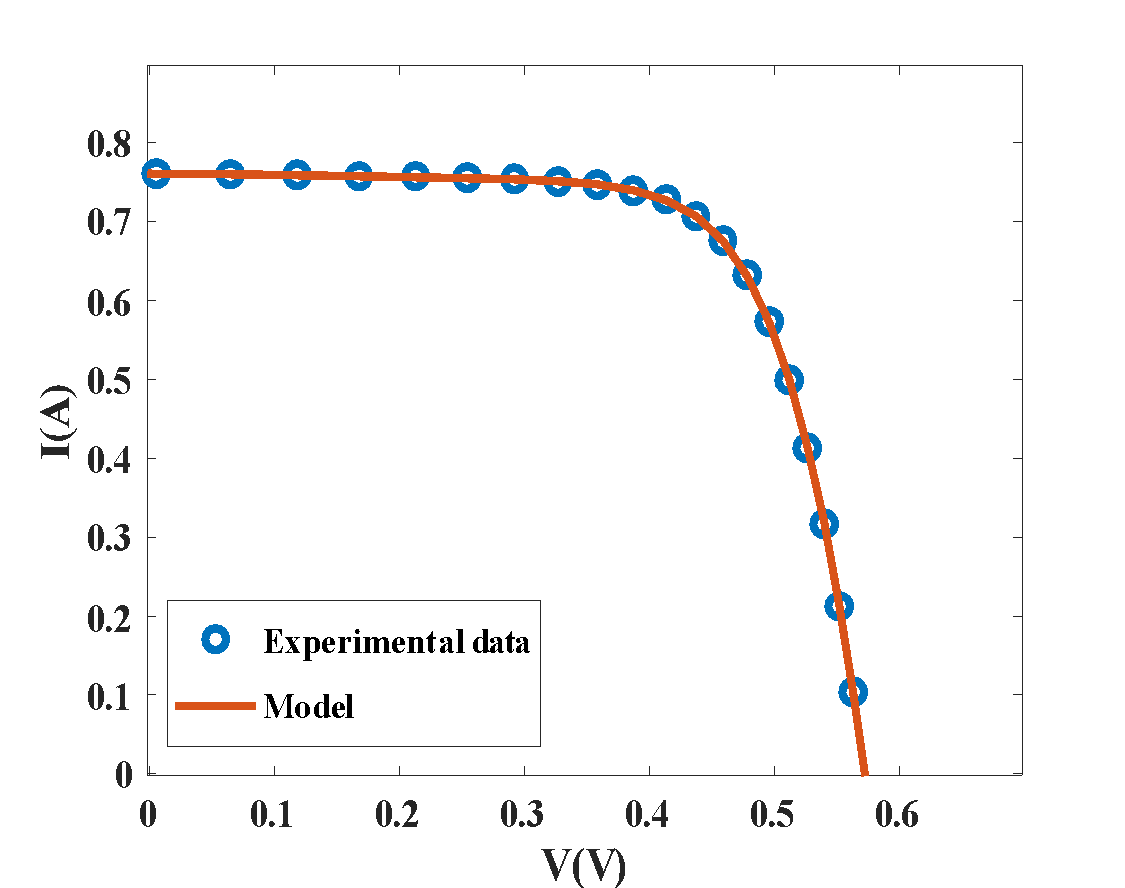
\includegraphics[scale=0.26 ]{Figure1}
%% make sure to add \vspace{.7em} before figure's caption
\vspace{.7em}
\caption{The architecture of MPLS network}
\end{figure}

\begin{table}[H]
\centering
\fontsize{8pt}{10pt}\selectfont
\caption{The performance of ...}
\begin{tabular}{ccc}
\hline
Variable & Speed (rpm) & Power (kW) \\
\hline
x & 10 & 8.6 \\
y & 15 & 12.4 \\
z & 20 & 15.3 \\
\hline
\end{tabular}
\end{table}

\begin{figure}[H]
	\centering
	\subfloat[]{
		\hspace{-2cm}
		\begin{minipage}[c][]{0.5\textwidth}
			\centering
			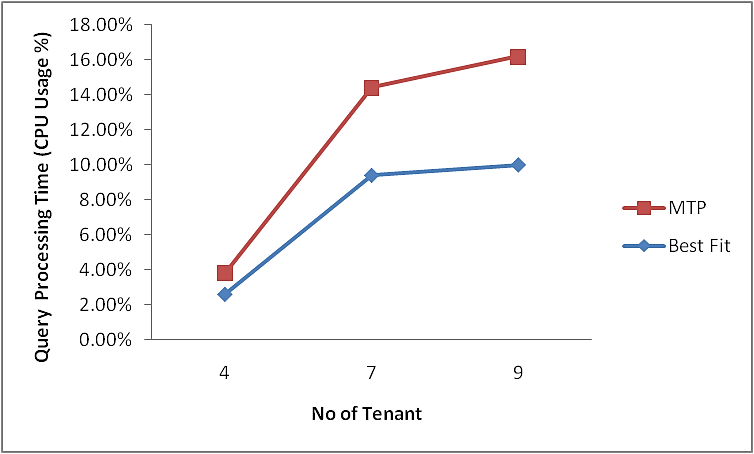
\includegraphics[width=10cm]{Figure2a}
	\end{minipage}}\\
	\subfloat[]{
		\hspace{-2cm}
		\begin{minipage}[c][]{0.5\textwidth}
			\centering
			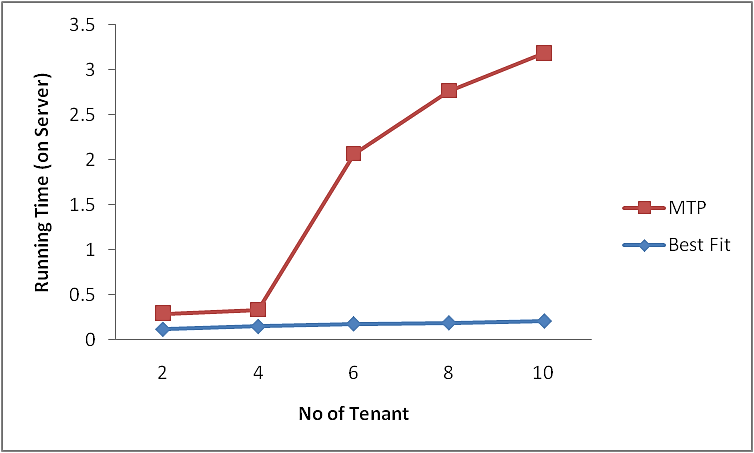
\includegraphics[width=10cm]{Figure2b}
	\end{minipage}}
	%% make sure to add \vspace{.7em} before figure's caption
	\vspace{.7em}
	\caption{Variation of average repeater spacing RR, km against (a) number of links and 
		(b) initial Raman pump wavelength}
\end{figure}

\section{Results and Discussion}
\label{}
This section explains the results of research and at the same time is given the comprehensive discussion. Results can be presented in figures, graphs, tables and others that make the reader understand easily [14], [15]. The discussion can be made in several sub-sections.

\subsection{Sub section 1}
Equations should be placed at the center of the line and provided consecutively with equation numbers in parentheses flushed to the right margin, as in (1). The use of Microsoft Equation Editor or MathType is preferred. All symbols that have not been mentioned in the equation should be explained in the following text.

\begin{equation}
E_v - E = \frac{\hbar}{2.m}(k_x^2 + k_y^2)
\end{equation}
%% make sure to add \vspace{.005em} after the end of equation


\subsection{Sub section 2}
Proper citation of other works should be made to avoid plagiarism. When referring to a reference item, please use the reference number as in [16] or [17] for multiple references. The use of ”Ref [18]...” should be employed for any reference citation at the beginning of sentence. For any reference with more than 3 or more authors, only the first author is to be written followed by \emph{et al.} (e.g. in [19]). Examples of reference items of different categories shown in the References section. Each item in the references section should be typed using 8 pt font size [20]–[25].

\subsubsection {Subsub section 1}
yy

\subsubsection {Subsub section 2}
zz

\section{Conclusion}
\label{}
Provide a statement that what is expected, as stated in the "INTRODUCTION" section can ultimately result in "RESULTS AND DISCUSSION" section, so there is compatibility. Moreover, the prospects for the development of research results and the application of further studies can also be added to the next (based on the results and discussion).

\section*{ACKNOWLEDGMENTS (if applicable)}
\label{}
This section should acknowledge individuals who provided personal assistance to the work but do not meet the criteria for authorship, detailing their contributions. It is imperative to obtain consent from all individuals listed in the acknowledgments.

\section*{FUNDING INFORMATION (mandatory)}
\label{}
This section should describe sources of funding agency that have supported the work. Authors should state how the research described in their article was funded, including grant numbers if applicable. Include the following (or similar) statement if there is no funding involved: Authors state no funding involved.

\section*{AUTHOR CONTRIBUTIONS STATEMENT (mandatory)}
\label{}
This journal uses the Contributor Roles Taxonomy (CRediT) to recognize individual author contributions, reduce authorship disputes, and facilitate collaboration. \textbf{The recommended number of authors is at least two, with one of them designated as the corresponding author.} The corresponding author will be responsible for all correspondence related to the paper and must ensure that the other authors are included in the communication regarding submission, revision, and publication processes. We encourage authors to include a statement in the paper that shares and accurately describes each author's contribution. \textbf{To be eligible for authorship, each individual must have contributed to at least one of the following: conceptualization, methodology, formal analysis, or investigation, as well as at least one aspect of writing (either original draft preparation or writing reviews and editing).}

\begin{table}[H]
	\centering
	\selectfont
	\begin{tabular}{lcccccccccccccc}
		\hline
		\textbf{Name of Author}\quad\quad\quad\quad\quad\quad\quad & \cellcolor[HTML]{D8F0F8}\textbf{C} & \cellcolor[HTML]{D8F0F8}\textbf{M} & \textbf{So} & \textbf{Va} & \cellcolor[HTML]{D8F0F8}\textbf{Fo} & \cellcolor[HTML]{D8F0F8}\textbf{I} & \textbf{R} & \textbf{D} & \cellcolor[HTML]{FDE9D9}\textbf{O} & \cellcolor[HTML]{FDE9D9}\textbf{E} & \textbf{Vi} & \textbf{Su} & \textbf{P} & \textbf{Fu} \\
		\hline
		Author 1 name & \cellcolor[HTML]{D8F0F8}\checkmark & \cellcolor[HTML]{D8F0F8}\checkmark & \checkmark & \checkmark & \cellcolor[HTML]{D8F0F8}\checkmark & \cellcolor[HTML]{D8F0F8}\checkmark &  & \checkmark & \cellcolor[HTML]{FDE9D9}\checkmark & \cellcolor[HTML]{FDE9D9}\checkmark &  &  & \checkmark &  \\
		Author 2 name &  \cellcolor[HTML]{D8F0F8}& \cellcolor[HTML]{D8F0F8}\checkmark &  &  & \cellcolor[HTML]{D8F0F8} & \cellcolor[HTML]{D8F0F8}\checkmark &  & \checkmark & \cellcolor[HTML]{FDE9D9}\checkmark & \cellcolor[HTML]{FDE9D9}\checkmark & \checkmark & \checkmark &  &  \\
		Author 3 name & \cellcolor[HTML]{D8F0F8}\checkmark & \cellcolor[HTML]{D8F0F8} & \checkmark & \checkmark & \cellcolor[HTML]{D8F0F8} & \cellcolor[HTML]{D8F0F8}\checkmark &  &  & \cellcolor[HTML]{FDE9D9}\checkmark & \cellcolor[HTML]{FDE9D9} & \checkmark &  & \checkmark & \\
		... & \cellcolor[HTML]{D8F0F8} & \cellcolor[HTML]{D8F0F8} &  &  &\cellcolor[HTML]{D8F0F8} & \cellcolor[HTML]{D8F0F8} &  &  & \cellcolor[HTML]{FDE9D9} & \cellcolor[HTML]{FDE9D9} &  &  &  & \\
		Author x name & \cellcolor[HTML]{D8F0F8} & \cellcolor[HTML]{D8F0F8} &  &  & \cellcolor[HTML]{D8F0F8}\checkmark & \cellcolor[HTML]{D8F0F8} &\checkmark &  & \cellcolor[HTML]{FDE9D9} & \cellcolor[HTML]{FDE9D9}\checkmark &  & \checkmark &  & \checkmark\\
		\hline
		\multicolumn{15}{c}{
			\begin{tabular}{llllll}
				&&&&&\\
				C &: 	\textbf{C}\fontsize{8}{10}\selectfont onceptualization \quad\quad\quad\quad\quad\quad\quad\quad& I &: 	\textbf{I}\fontsize{8}{10}\selectfont nvestigation & Vi&: 	\textbf{Vi}\fontsize{8}{10}\selectfont sualization  \\
				M &: 	\textbf{M}\fontsize{8}{10}\selectfont ethodology & R &: 	\textbf{R}\fontsize{8}{10}\selectfont esources & Su&: 	\textbf{Su}\fontsize{8}{10}\selectfont pervision  \\
				So&: 	\textbf{So}\fontsize{8}{10}\selectfont ftware & D &:	\textbf{D}\fontsize{8}{10}\selectfont ata Curation & P &: 	\textbf{P}\fontsize{8}{10}\selectfont roject Administration  \\
				Va&: 	\textbf{Va}\fontsize{8}{10}\selectfont lidation & O &:	\fontsize{8}{10}\selectfont Writing - \fontsize{10}{12}\selectfont \textbf{O}\fontsize{8}{10}\selectfont riginal Draft & Fu&: 	\textbf{Fu}\fontsize{8}{10}\selectfont nding Acquisition \\
				Fo&: 	\textbf{Fo}\fontsize{8}{10}\selectfont rmal Analysis & E &:	\fontsize{8}{10}\selectfont Writing - Review \& \fontsize{10}{12}\selectfont\textbf{E}\fontsize{8}{10}\selectfont diting \quad\quad\quad\quad\quad\quad\quad&  \\
			\end{tabular}
		}
	\end{tabular}
\end{table}



\newpage\noindent See the examples below:
\begin{table}[H]
	\centering
	\selectfont
	\begin{tabular}{lcccccccccccccc}
		\hline
		\textbf{Name of Author} & \cellcolor[HTML]{D8F0F8}\textbf{C} & \cellcolor[HTML]{D8F0F8}\textbf{M} & \textbf{So} & \textbf{Va} & \cellcolor[HTML]{D8F0F8}\textbf{Fo} & \cellcolor[HTML]{D8F0F8}\textbf{I} & \textbf{R} & \textbf{D} & \cellcolor[HTML]{FDE9D9}\textbf{O} & \cellcolor[HTML]{FDE9D9}\textbf{E} & \textbf{Vi} & \textbf{Su} & \textbf{P} & \textbf{Fu} \\
		\hline
		Zahra Pezeshki & \cellcolor[HTML]{D8F0F8}\checkmark & \cellcolor[HTML]{D8F0F8}\checkmark & \checkmark & \checkmark & \cellcolor[HTML]{D8F0F8}\checkmark &\cellcolor[HTML]{D8F0F8} \checkmark &  & \checkmark & \cellcolor[HTML]{FDE9D9}\checkmark &\cellcolor[HTML]{FDE9D9} \checkmark &  &  & \checkmark &  \\
		Tanweer Alam & \cellcolor[HTML]{D8F0F8} & \cellcolor[HTML]{D8F0F8}\checkmark &  &  & \cellcolor[HTML]{D8F0F8} & \cellcolor[HTML]{D8F0F8}\checkmark &  & \checkmark &\cellcolor[HTML]{FDE9D9} \checkmark & \cellcolor[HTML]{FDE9D9}\checkmark & \checkmark & \checkmark &  &  \\
		Laith Mohammad Abualigah& \cellcolor[HTML]{D8F0F8}\checkmark &\cellcolor[HTML]{D8F0F8}  & \checkmark & \checkmark & \cellcolor[HTML]{D8F0F8} & \cellcolor[HTML]{D8F0F8}\checkmark &  &  & \cellcolor[HTML]{FDE9D9}\checkmark &\cellcolor[HTML]{FDE9D9}  & \checkmark &  & \checkmark & \checkmark\\
		\hline
	\end{tabular}
\end{table}

\section*{CONFLICT OF INTEREST STATEMENT (mandatory)}
\label{}
To ensure fair and objective decision-making, authors must declare any associations that pose a conflict of interest (financial, personal, or professional) in connection with manuscripts. Non-financial competing interests include a declaration of political, personal, religious, ideological, academic, and intellectual competing interests. The authors declare that they have no known competing financial interests or personal relationships that could have appeared to influence the work reported in this paper. If there are no conflicts of interest, please include the following author's statement: Authors state no conflict of interest.

\section*{INFORMED CONSENT (if applicable)}
\label{}
The protection of privacy is a legal right that must not be breached without individual informed consent. In cases where the identification of personal information is necessary for scientific reasons, authors should obtain full documentation of informed consent, including written permission from the patient prior to inclusion in the study. Incorporate the following (or a similar) statement: We have obtained informed consent from all individuals included in this study.

\section*{ETHICAL APPROVAL (if applicable)}
\label{}
When papers talk about using people or animals, authors should make it clear that the research followed all national rules and institutional policies, and it was approved by the authors' institutional review board or a similar committee. The Helsinki Declaration's tenets must guide all investigations involving human subjects. Authors must also identify the committee or review board approving the experiments and provide a statement indicating approval of the research. Incorporate the following (or a similar) statement: The research related to human use has been complied with all the relevant national regulations and institutional policies in accordance with the tenets of the Helsinki Declaration and has been approved by the authors' institutional review board or equivalent committee; or: The research related to animal use has been complied with all the relevant national regulations and institutional policies for the care and use of animals.

\section*{DATA AVAILABILITY (mandatory)}
\label{}
The data availability statement is a valuable link between a paper’s results and the supporting evidence. It is a brief statement about whether the authors of an article have made the evidence supporting their findings available, and if so, where readers may access it. Data availability statements help to promote transparency and reproducibility in research and to increase the visibility of valuable evidence produced or gathered during the course of research. As part of our commitment to supporting open research, our journal now requires all manuscripts to include a data availability statement in order to be accepted for publication. Examples:
\begin{itemize}[topsep=0.3ex, itemsep=0.3ex, parsep=0.2ex]
	\item[-] The supporting data of this study are openly available in [repository's name] at http://doi.org/[doi], reference number [reference number].
	\item[-] The data that support the findings of this study will be available in [repository's name] [URL / DOI link] following a [6 month] embargo from the date of publication to allow for the commercialization of research findings.
	\item[-] The data that support the findings of this study are available on request from the corresponding author, [initials: AB]. The data, which contain information that could compromise the privacy of research participants, are not publicly available due to certain restrictions.
	\item[-] Derived data supporting the findings of this study are available from the corresponding author [initials: AB] on request.
	\item[-] The data that support the findings of this study are available from [third party]. Restrictions apply to the availability of these data, which were used under license for this study. Data are available [from the authors / at URL] with the permission of [third party].
	\item[-] The authors confirm that the data supporting the findings of this study are available within the article [and/or its supplementary materials].
	\item[-] The data that support the findings of this study are available from the corresponding author, [initials: AB], upon reasonable request.
	\item[-] Data availability is not applicable to this paper as no new data were created or analyzed in this study.
\end{itemize}


\section*{REFERENCES}
\label{}
\footnotesize
The main references are international journals and proceedings. All references should be to the most pertinent, up-to-date sources, \textbf{and the minimum number of references} should be \textbf{25} (for original research papers) and \textbf{50} (for review papers). References are written in IEEE style. You can access a more comprehensive guide at http://ipmuonline.com/guide/refstyle.pdf. Use a tool such as EndNote, Mendeley, or Zotero for reference management and formatting; choose \textbf{IEEE style}. Please use a consistent format for references—see examples (8 pt):

\subsection*{[1] Journal/Periodicals}
\footnotesize
\begin{flushleft}
\textsl{Basic Format:\\}
\end{flushleft}
\vspace{-1.1em} 
J. K. Author, “Title of paper,” \textsl{Abbrev. Title of Journal/Periodical}, vol. x, no. x, pp. xx-xx, Abbrev. Month, year, doi: xxx.\\ 
\emph{Examples:}
\begin{enumerate} [leftmargin=*, topsep=0.3ex, itemsep=0.3ex, parsep=0.2ex]
\footnotesize
\item[$-$] M. M. Chiampi and L. L. Zilberti, “Induction of electric field in human bodies moving near MRI: An efficient BEM computational procedure,” \textsl{IEEE Transaction on Biomedical Engineering}, vol. 58, pp. 2787–2793, Oct. 2011, doi: 10.1109/TBME.2011.2158315.
\item[$-$] R. Fardel, M. Nagel, F. Nuesch, T. Lippert, and A. Wokaun, “Fabrication of organic light emitting diode pixels by laser-assisted forward transfer,” \textsl{Appl. Phys. Lett.}, vol. 91, no. 6, Aug. 2007, Art. no. 061103, doi: 10.1063/1.2759475.
\end{enumerate}


\subsection*{[2]	Conference Proceedings}
\footnotesize
\begin{flushleft}
\textsl{Basic Format:\\}
\end{flushleft}
\vspace{-1.1em} 
J. K. Author, “Title of paper,” \textsl{in Abbreviated Name of Conf.}, (location of conference is optional), year, pp. xxx–xxx, doi: xxx. \\
\emph{Examples:}
\begin{enumerate} [leftmargin=*, topsep=0.3ex, itemsep=0.3ex, parsep=0.2ex]
\footnotesize
\item[$-$] G. Veruggio, “The EURON roboethics roadmap,” in \textsl{Proc. Humanoids ’06: 6th IEEE-RAS Int. Conf. Humanoid Robots}, 2006, pp. 612–617, doi: 10.1109/ICHR.2006.321337. 
\item[$-$]	J. Zhao, G. Sun, G. H. Loh, and Y. Xie, “Energy-efficient GPU design with reconfigurable in-package graphics memory,” in \textsl{Proc. ACM/IEEE Int. Symp. Low Power Electron. Design (ISLPED)}, Jul. 2012, pp. 403–408, doi: 10.1145/2333660.2333752.
\end{enumerate}


\subsection*{[3] Book}
\footnotesize
\begin{flushleft}
\textsl{Basic Format:\\}
\end{flushleft}
\vspace{-1.1em} 
\footnotesize
J. K. Author, “Title of chapter in the book,” in \textsl{Title of His Published Book}, X. Editor, Ed., xth ed. City of Publisher, State (only U.S.), Country: Abbrev. of Publisher, year, ch. x, sec. x, pp. xxx–xxx. \\
\textsl{Examples:}
\begin{enumerate} [leftmargin=*, topsep=0.3ex, itemsep=0.3ex, parsep=0.2ex]
\footnotesize
    \item[$-$] A. Taflove, \textsl{Computational Electrodynamics: The Finite-Difference Time-Domain Method} in Computational Electrodynamics II, vol. 3, 2nd ed. Norwood, MA, USA: Artech House, 1996. 
		\item[$-$] R. L. Myer, “Parametric oscillators and nonlinear materials,” in \textsl{Nonlinear Optics}, vol. 4, P. G. Harper and B. S. Wherret, Eds., San Francisco, CA, USA: Academic, 1977, pp. 47–160.
\end{enumerate}


%% References
%%
%% Following citation commands can be used in the body text:
%% Usage of \cite is as follows:
%%   \cite{key}         ==>>  [#]
%%   \cite[chap. 2]{key} ==>> [#, chap. 2]
%%

%% References with BibTeX database:

\bibliographystyle{IEEEtran}
%\bibliography{<your-bib-database>}
%% Authors are advised to use a BibTeX database file for their reference list.
%% The provided style IEEEtran.bst formats references is generally used.

%% For references without a BibTeX database:

\begin{thebibliography} {99} 
\footnotesize
\itemsep 0pt 


%%The main references are international journals and proceedings. All references should be to the most pertinent, up-to-date sources and the minimum of references are 25. References are written in IEEE style. Please use a consistent format for references – see examples below:

%% \bibitem must have the following form:
%%   \bibitem{key}...
%%

 \bibitem{1} A. Chakraborty and A. K. Kar, “Swarm Intelligence: A Review of Algorithms,” in \textsl{Nature-Inspired Comput. Optim. Model. Optim. Sci. Technol.,} Springer, 2017, pp. 475–494.

\bibitem{2} Q. Li \textsl{et al.}, “An Enhanced Grey Wolf Optimization Based Feature Selection Wrapped Kernel Extreme Learning Machine for Medical Diagnosis,” \textsl{Comput. Math. Methods Med.}, vol. 2017, pp. 1–15, 2017, doi: 10.1155/2017/9512741.

\bibitem{3} N. M. Arzeno, Z.-D. Deng, and C.-S. Poon, “Analysis of First-Derivative Based QRS Detection Algorithms,” \textsl{IEEE Trans. Biomed. Eng.}, vol. 55, no. 2, pp. 478–484, Feb. 2008, doi: 10.1109/TBME.2007.912658.

\bibitem{4} W. Pieters, “Acceptance of Voting Technology: Between Confidence and Trust,” in \textsl{Int. Conf. Trust Manag.}, 2006, pp. 283–297, doi: 10.1007/11755593\_21.

\bibitem{5} G. M. Friesen, T. C. Jannett, M. A. Jadallah, S. L. Yates, S. R. Quint, and H. T. Nagle, “A comparison of the noise sensitivity of nine QRS detection algorithms,” \textsl{IEEE Trans. Biomed. Eng.}, vol. 37, no. 1, pp. 85–98, 1990, doi: 10.1109/10.43620.

\bibitem{6} P. S. Hamilton and W. J. Tompkins, “Compression of the ambulatory ECG by average beat subtraction and residual differencing,” \textsl{IEEE Trans. Biomed. Eng.}, vol. 38, no. 3, pp. 253–259, Mar. 1991, doi: 10.1109/10.133206.

\bibitem{7} M. Achieng and E. Ruhode, “The Adoption and Challenges of Electronic Voting Technologies Within the South African Context,” \textsl{Int. J. Manag. Inf. Technol.}, vol. 5, no. 4, pp. 1–12, Nov. 2013, doi: 10.5121/ijmit.2013.5401.

\bibitem{8} D. Cansell, J. P. Gibson, and D. Méry, “Refinement: A Constructive Approach to Formal Software Design for a Secure e-voting Interface,” \textsl{Electron. Notes Theor. Comput. Sci.}, vol. 183, pp. 39–55, Jul. 2007, doi: 10.1016/j.entcs.2007.01.060.

\bibitem{9} M. Hapsara, A. Imran, and T. Turner, “Beyond Organizational Motives of e-Government Adoption: The Case of e-Voting Initiative in Indonesian Villages,” \textsl{Procedia Comput. Sci.}, vol. 124, pp. 362–369, 2017, doi: 10.1016/j.procs.2017.12.166.

\bibitem{10} BM. F.M.Mursi, G. M. R. Assassa, A. Abdelhafez, and K. M. Abo Samra, “On the Development of Electronic Voting: A Survey,” \textsl{Int. J. Comput. Appl.}, vol. 61, no. 16, pp. 1–11, Jan. 2013, doi: 10.5120/10009-4872.

\bibitem{11} K. Vassil, M. Solvak, P. Vinkel, A. H. Trechsel, and R. M. Alvarez, “The diffusion of internet voting. Usage patterns of internet voting in Estonia between 2005 and 2015,” \textsl{Gov. Inf. Q.}, vol. 33, no. 3, pp. 453–459, Jul. 2016, doi: 10.1016/j.giq.2016.06.007.

\bibitem{12} F. Zhang and Y. Lian, “QRS Detection Based on Multiscale Mathematical Morphology for Wearable ECG Devices in Body Area Networks,” \textsl{IEEE Trans. Biomed. Circuits Syst.}, vol. 3, no. 4, pp. 220–228, Aug. 2009, doi: 10.1109/TBCAS.2009.2020093.

\bibitem{13} N. Valaei, S. R. Nikhashemi, H. Ha Jin, and M. M. Dent, “Task Technology Fit in Online Transaction Through Apps,” in \textsl{Optimizing E-Participation Initiatives Through Social Media}, IGI Global, 2018, pp. 236–251.

\bibitem{14} M. Merri, D. C. Farden, J. G. Mottley, and E. L. Titlebaum, “Sampling frequency of the electrocardiogram for spectral analysis of the heart rate variability,” \textsl{IEEE Trans. Biomed. Eng.}, vol. 37, no. 1, pp. 99–106, 1990, doi: 10.1109/10.43621.

\bibitem{15} T. J. McGill and J. E. Klobas, “A task–technology fit view of learning management system impact,” \textsl{Comput. Educ.}, vol. 52, no. 2, pp. 496–508, Feb. 2009, doi: 10.1016/j.compedu.2008.10.002.

\bibitem{16} B. Furneaux, “Task-Technology Fit Theory: A Survey and Synopsis of the Literature,” in \textsl{Information Systems Theory,} Springer, 2012, pp. 87–106.

\bibitem{17} E. M. H. Saeed and H. A. Saleh, “Pectoral Muscles Removal in Mammogram Image by Hybrid Bounding Box and Region Growing Algorithm,” in \textsl{2020 Int. Conf.  Comput. Sci. Softw. Eng. (CSASE)}, Apr. 2020, pp. 146–151, doi: 10.1109/CSASE48920.2020.9142055.

\bibitem{18} D. L. Goodhue and R. L. Thompson, “Task-Technology Fit and Individual Performance,” \textsl{MIS Q.}, vol. 19, no. 2, pp. 213–233, Jun. 1995, doi: 10.2307/249689.

\bibitem{19} S. Mostafa, R. Mubarak, M. El-Adawy, A. F. Ibrahim, M. M. Gomaa, and R. M. Kamal, “Breast Cancer Detection Using Polynomial Fitting Applied on Contrast Enhanced Spectral Mammography,” in \textsl{2019 Int. Conf. Innov. Trends Comput. Eng. (ITCE)}, Feb. 2019, pp. 11–16, doi: 10.1109/ITCE.2019.8646379.

\bibitem{20} A. Tharwat, “Classification assessment methods,” \textsl{Appl. Comput. Informatics}, vol. 17, no. 1, pp. 168–192, Jan. 2021, doi: 10.1016/j.aci.2018.08.003.

\bibitem{21} A. Sahu and S. Pattnaik, “Feature Selection Using Evolutionary Functional Link Neural Network for Classification,” \textsl{Int. J. Adv. Appl. Sci.}, vol. 6, no. 4, pp. 359–367, Dec. 2017, doi: 10.11591/ijaas.v6.i4.pp359-367.

\bibitem{22} W. Zikmund, B. J. Babin, J. C. Carr, and M. Griffin, \textsl{Business Research Methods Eight Edition}. Canada: Nelson Education, 2010.

\bibitem{23} S. Soegijoko, I. M. Puspitasari, A. Aridarma, and I. D. Jani, “e-health for improving community healthcare: Encouraging clinical experience of simple e-prescription system and m-health system development for mother and childcare,” in \textsl{2011 IEEE 13th Int. Conf. e-Health Netw., Appl. Services (Healthcom)}, Jun. 2011, pp. 102–105, doi: 10.1109/HEALTH.2011.6026722.

\bibitem{24} M. Mishra, V. K. Mishra, and H. R. Sharma, “Leveraging knowledge based question answer technology to address user-interactive short domain question in natural language,” in \textsl{2012 2nd Nat. Conf. Comput. Intell. Signal Process. (CISP)}, Mar. 2012, pp. 86–90, doi: 10.1109/NCCISP.2012.6189683.

\bibitem{25} Z. Denan, Z. A. Munir, R. A. Razak, K. Kamaruddin, and V. Pandiyan Kaliani Sundram, “Adoption of technology on E-learning effectiveness,” \textsl{Bull. Electr. Eng. Informatics}, vol. 9, no. 3, pp. 1121–1126, Jun. 2020, doi: 10.11591/eei.v9i3.1717.

 \end{thebibliography}

\section*{BIOGRAPHIES OF AUTHORS} 
\normalsize
In this section, authors are required to provide their professional biography, which should include their academic background, current position, research interests, and any significant contributions to the current study. Additionally, authors should include links to their professional profiles, such as ORCID iD (mandatory) and, if applicable, Google Scholar, Scopus Author ID, or Web of Science (WoS) ResearcherID. This helps establish the author’s academic identity and enhances the visibility of their research.

\noindent Required Information:
\begin{itemize}[topsep=0.3ex, itemsep=0.3ex, parsep=0.2ex]
	\item[-] Full name: Include the author's full name as it appears in official records. If preferred, authors may use the format consistent with his/her Scopus profile.
	\item[-] Email address for each author: Provide the author's professional email address to facilitate correspondence.
	\item[-] Social media account:
	\begin{itemize}[topsep=0.3ex, itemsep=0.3ex, parsep=0.2ex]
		\item[$\blacksquare$] ORCID iD: This is a mandatory. Each author must include their ORCID iD (https://orcid.org/), which helps link his/her research output to their identity.
		\item[$\blacksquare$] Google Scholar Profile: Include the link to the author's Google Scholar profile. If the author does not have a Google Scholar profile, they may create a new one and include the link.
		\item[$\blacksquare$] Scopus Author ID: If available, include the Scopus Author ID to enhance visibility on Scopus.
		\item[$\blacksquare$] Web of Science (WoS) ResearcherID: Include the Web of Science ResearcherID. If the author does not have a WoS profile, they may create a new one and include the link.
	\end{itemize}
	\item[-] Brief biography: Provide a concise overview of the author's academic background, research interests, notable publications, and contributions to the current paper. This should be no longer than 150 to 200 words (9 pt).
	\item[-] Professional achievements: If available, mention any important awards, recognition, or research projects the author has been involved in.
	\item[-] Photo Submission: Authors must submit a clear, professional headshot (3x4 cm). The photo should be of high quality, well-lit, and not blurry. Avoid using photos that are overly casual or low resolution.
\end{itemize}


\noindent Below is an example of how to format the biography section for each author:

\section*{BIOGRAPHIES OF AUTHORS}
%% make sure to add \vspace{-.7em} before \begin{biography}
\vspace{-.7em} 
\small
\begin{biography}[{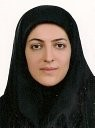
\includegraphics[width=2.5cm,height=4cm,clip,keepaspectratio]{Author1}}]
\textbf{Zahra Pezeshki} %% Affiliation and educational background.
\href{https://orcid.org/0000-0003-3366-3647}{
\includegraphics[width=0.02\textwidth]{orcid.png}} 
\href{https://scholar.google.com/citations?user=XKJhK78AAAAJ&hl=en}{
\includegraphics[width=0.02\textwidth]{gscholar.png}}
\href{https://www.scopus.com/authid/detail.uri?authorId=57191962990}{
\includegraphics[width=0.02\textwidth]{scopus.png}}
\href{https://www.webofscience.com/wos/author/rid/E-1666-2017/}{
\includegraphics[width=0.02\textwidth]{wos.png}} is a master's holder in Electrical Engineering-Electronics Integrated Circuitsfrom the Shahrood University of Technology, Faculty of Electrical and Robotics Engineering where she presented a new method for energy consumption improvement by determination of the best location for cooling and heating appliances in buildings. She has worked as a lecturer, instructor, and adjunct professor with companies, academies, and universities. She has reviewed for 23 double-blind peer reviews. She has worked as an invited researcher with national and international universities. Her broad research interests cover topics relating to electrical and electronics, computer, energy, mechanics, chemistry, civil, and physics. She can be contacted at email: tejaratemrooz@gmail.com.
\end{biography}

\vspace{.7em}

\begin{biography}[{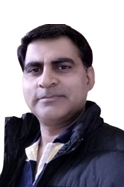
\includegraphics[width=2.5cm,height=4cm,clip,keepaspectratio]{Author2}}]
\textbf{Tanweer Alam} %% Affiliation and educational background.
\href{https://orcid.org/0000-0003-2731-4627}{
\includegraphics[width=0.02\textwidth]{orcid.png}} 
\href{https://scholar.google.com/citations?user=MUQy5QUAAAAJ&hl=id&oi=ao}{
\includegraphics[width=0.02\textwidth]{gscholar.png}}
\href{https://www.scopus.com/authid/detail.uri?authorId=57189067051}{
\includegraphics[width=0.02\textwidth]{scopus.png}}
\href{https://www.webofscience.com/wos/author/rid/M-7780-2017/}{
\includegraphics[width=0.02\textwidth]{wos.png}} is working in Islamic University of Madinah as a Professor (Associate). His academic qualification is Ph.D., MPhil, MTech, MCA, MSc. His research area includes Blockchain, Internet of Things and Wireless Communications. His profile was published in Who’s who in the world- 2013. He has membership of IACSIT, IAEngg, ISOC, Computer Science Teachers Association etc. He is a single author of twelve books. His books are included in the curriculum of several universities. He can be contacted at email: tanweer03@iu.edu.sa.
\end{biography}

\vspace{.7em}

\begin{biography}
[{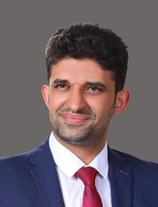
\includegraphics[width=2.5cm,height=4cm,clip,keepaspectratio]{Author3}}]
\textbf{Laith Mohammad Abualigah} %% Affiliation and educational background.
\href{https://orcid.org/0000-0002-2203-4549}{
\includegraphics[width=0.02\textwidth]{orcid.png}} 
\href{https://scholar.google.com/citations?user=39g8fyoAAAAJ&hl=id&oi=sra}{
\includegraphics[width=0.02\textwidth]{gscholar.png}}
\href{https://www.scopus.com/authid/detail.uri?authorId=57190984712}{
\includegraphics[width=0.02\textwidth]{scopus.png}}
\href{https://www.webofscience.com/wos/author/rid/ABC-9695-2020/}{
\includegraphics[width=0.02\textwidth]{wos.png}} received his first degree from Al-Albayt University, Computer Information System, Jordan, in 2011. He has also Master degree from Al-Albayt University, Computer Science, Jordan, in 2014. The Ph.D. degree from the School of Computer Science in Universiti Sains Malaysia (USM), Malaysia in 2018. He is currently a computer science researcher. His main research interests focus on Bio-inspired Computing, Artificial Intelligence, Metaheuristic Modeling and Optimization, Evolutionary Computations, Optimization algorithms, Information Retrieval, Feature Selection, Combinatorial Problems, Data Mining, and Text Mining. He can be contacted at email: lx.89@yahoo.com..
\end{biography}
\newpage

\end{document}
%%
%% End of file `iaesarticle.tex'. 